\documentclass{jsarticle}
\usepackage{amssymb,amsmath,amsthm}
\usepackage{newtxtt}
\usepackage[utf8]{inputenc}
\usepackage[dvipdfmx]{graphicx}
\usepackage{here}
\newcommand{\kakko}[1][]{(#1)}
\newcommand{\bx}{\mathbf{x}}
\newcommand{\bv}{\mathbf{v}}
\newcommand{\bb}{\mathbf{b}}
\newcommand{\bd}{\mathbf{d}}
\newcommand{\pder}[2][]{\frac{\partial#1}{\partial#2}}
\newcommand{\dder}[2][]{\frac{\mathrm{d}#1}{\mathrm{d}#2}}
\newcommand{\ddder}[2][]{\frac{\mathrm{d^2}#1}{\mathrm{d}#2^2}}
\newcommand{\Dder}[2][]{\frac{\mathrm{D}#1}{\mathrm{D}#2}}
\newcommand{\half}{\frac{1}{2}}
\newcommand{\hpn}{n + \half}
\newcommand{\hmn}{n - \half}
\newcommand{\hpj}{j + \half}
\newcommand{\hml}{j - \half}
\newcommand{\hpi}{i + \half}
\newcommand{\hmi}{i - \half}
\newcommand{\ethe}{E_{th}}
\newcommand{\beq}{\begin{equation}}
\newcommand{\beql}[1]{\begin{equation}\label{#1}}
\newcommand{\eeq}{\end{equation}}
\newcommand{\eeqp}{\;\;\;.\end{equation}}
\newcommand{\eeqc}{\;\;\;,\end{equation}}
\newcommand{\xid}{x_i^2}
\newcommand{\lid}{l_i^2}
\newcommand{\aid}{a_i^2}

\renewcommand{\theequation}{\thesection.\arabic{equation}}
\makeatletter
\@addtoreset{equation}{section}
\makeatother

\date{\today}
\author{山田龍}
\title{原始星形成の1次元数値計算}
\begin{document}
\maketitle
\section{Introduction}
\subsection{星形成の概要}
星形成領域にはRho Ophiuchi, Taurus Molecular Cloud, Orion Nebulaなどがある。
(写真はる)
%https://en.wikipedia.org/wiki/List_of_star-forming_regions_in_the_Local_GroupF
%https://www-tap.scphys.kyoto-u.ac.jp/~hosokawa/download/%E5%A4%A9II8.pdf
星形成領域はフィラメントのような構造をしていることもある。
原始星(質量が有意に増えつつある星)が形成されると、原始星への降着は数万年程度続く。
質量が1$M_\odot$に達すると、質量降着が止まる。
%表現変える
質量降着が終わると、1$M_\odot$の星は林トラックに乗ったあと、
ヘニエトラックに沿って進化する。そして、主系列星に至る。

\subsection{課題}
星形成の過程は、暗く冷たいガスの中で進むので直接観測することでできない。
具体的には、崩壊の過程において内部が暴走的に収縮をするので中心の進化が外から見えない。
一般に原始星の形成には数十万年かかる。
分子雲の中の重力崩壊を数値的に計算する研究が行われてきた。
とくに一次元での計算はLarson(1969)やMasunagaInutsuka(2000)による仕事がある。
まず、その仕事を再現する。
初期条件と観測される星のあいだのシナリオを検証する。

\section{Related Work}
\section{基礎理論}
\subsection{基礎方程式}
このレポートでは、自己重力と放射を入れた方程式を解く。
自己重力とは、流体に働く重力のうちの流体自身の作る重力のことである。
自己重力を除いた重力は外場として与えられる重力である。
支配方程式は以下のようになる :\\
連続の式
\begin{equation}
    \pder[\rho]{t} = - \nabla \bv
\end{equation}
運動方程式は単位質量あたりの重力ポテンシャルを$\Phi$として、
\begin{equation}
    \Dder[\bv]{t} = - \frac{1}{\rho}\nabla{p} - \nabla\Phi\label{eq:euler}
\end{equation}

エネルギー方程式は単位質量あたりの内部エネルギーを$e$、加熱率を$\gamma$、冷却率を$\lambda$として、
\begin{equation}
    \Dder[e]{t} = - \frac{p}{\rho} \nabla \cdot \bv + \Gamma - \lambda
\end{equation}
ここで、ラグランジュ微分は、流れに沿った微分で
\begin{equation}
    \Dder[]{t} = \pder[]{t} + \bv\pder[]{\bx}
\end{equation}
である。
また、重力ポテンシャルは重力定数を$G$として、ポアソン方程式の解として与えられる。
\beq
 \Delta \Phi = 4 \pi G \rho
\eeq
\subsubsection{連続の式の導出}
微小体積要素$\delta V = \delta x \delta y \delta z$を取ると、流れに沿って質量が保存する。
\begin{equation}
    \Dder[]{t} (\rho\delta V)= 0\label{eq:mass}
\end{equation}
\eqref{eq:mass}より、
\begin{align}
    %\rho\Dder[]{t} \delta V &+ \delta V\Dder[]{t} \rho= 0\\
    \Dder[\rho]{t} &= -\frac{\rho}{\delta V}\Dder[]{t} \delta V \\
    % &= -\frac{\rho}{ \delta x \delta y \delta z}\Dder[]{t}( \delta x \delta y \delta z)\\
     %&= -\rho(\frac{1}{\delta x}\Dder[\delta x]{t} + \frac{1}{\delta y}\Dder[\delta y]{t} + \frac{1}{\delta z}\Dder[\delta z]{t})\\
     %&= -\rho(\frac{1}{\delta x}\Dder[\delta x]{t} + \frac{1}{\delta y}\Dder[\delta y]{t} + \frac{1}{\delta z}\Dder[\delta z]{t})\\
     %&= -\rho(\frac{\delta u}{\delta x} + \frac{\delta v}{\delta y} + \frac{\delta w}{\delta z})\\
     &= - \rho \nabla \cdot \bv\\
    \pder[\rho]{t} &= -  \nabla \cdot (\rho\bv)\label{eq:continuous}
\end{align}
\label{eq:continuous}が連続の式である。
また、非圧縮性流体では$\nabla \cdot \bv = 0$であるから、連続の式は
\begin{equation}
    \pder[\rho]{t} = -  \rho \nabla \cdot \bv
\end{equation}
となる。
\subsubsection{運動方程式の導出}
微小体積要素に働く力は、重力ポテンシャルによる力と応力を考えて、
\begin{equation}
     \Dder[(\rho \delta V \bv)]{t} = - (\nabla p) \delta V - p \delta V \nabla \Phi
\end{equation}
左辺に質量保存則\eqref{eq:mass}を用いれば、運動方程式が導かれる。
\begin{equation}
    \Dder[\bv]{t} = - \frac{1}{\rho}\nabla p - \nabla\mathbf{\Phi}
\end{equation}
\subsubsection{運動エネルギーの保存則}
\subsubsection{TheRaynoldsTransportTheorem}
\subsubsection{エネルギー方程式の導出}
理想気体で孤立系を仮定して
エネルギー保存則
\beq
\Dder[]{t} \int \rho(e + \half v^2) dV = \int f \cdot v dV - \int pv \cdot n dS\label{eq:energysave}
\eeq
から出発する。
左辺は内部エネルギーと運動エネルギーの和の変化率で
右辺第一項は外力のする仕事率、第二項は表面で圧力のする仕事率である。
TheRaynoldsTransportTheoremを使って、
\beq
\Dder[]{t} \int \rho(e + \half v^2) dV  = \int \rho \Dder[]{t} (e + \half v^2)dV   
\eeq    
右辺第二項の表面積分を体積分に直して、
\beq
\int pv \cdot n dS = \int \nabla \cdot (pv) dV
\eeq
である。したがってエネルギー保存の式\eqref{eq:energysave}は
\beq
\int \rho \Dder[]{t} (e + \half v^2)dV =\int f \cdot v dV -  \int \nabla \cdot (pv) dV
\eeq
積分をまとめると、
\beq
    \rho \Dder[]{t} (e + \half v^2) + \nabla \cdot (pv) = f \cdot v
\eeq
ここから、
\beq
    \rho \Dder[]{t} v^2 = v \cdot f - (v \cdot \nabla) p
\eeq
を引いて
\beq
    \rho \Dder[]{t} e + p (\nabla \cdot v) = 0
\eeq
を得る。
\subsection{ビリアル定理}
%http://jun-makino.sakura.ne.jp/kougi/stellar_dynamics_2009/note3/node3.html
%http://th.nao.ac.jp/MEMBER/tomisaka/Lecture_Notes/StarFormation/6/node44.html#eqn:virial-2-5_3
重力と圧力勾配がつりあっていて、力学平衡にある系において、系の全重力エネルギー$W$とそして全内部エネルギー$E_{th}$には簡単な関係があり、ビリアル定理と呼ばれる。
\begin{equation}
     2E_{th} + W = 0
\end{equation}
ここでは、流体の自己重力系における力学平衡とは系の力学的性質が変化するタイムスケールが系の特徴的な時間である
自由落下時間に比べて大きいときに系が力学的平衡にあるという。
\subsubsection{ビリアル定理の導出}
運動方程式\eqref{eq:euler}の両辺に$\rho$をかけて整理すると、
\begin{align}
    \rho\Dder[v_i]{t} &= - \pder[p]{x_i} - \rho\pder[\Phi]{x_i}\\
    \pder[]{t}(\rho v_i) &= - \pder[]{x_j}(\rho v_iv_j) - \pder[p]{x_i} - \rho\pder[\Phi]{x_i}
\end{align}
両辺に$x_k$をかけて体積積分すれば、
\begin{align}
    \int d^3x x_k \pder[]{t}(\rho v_i) &= - \int d^3x x_k\pder[]{x_j}(\rho v_iv_j) - \int d^3x x_k\pder[p]{x_i} - \int d^3x x_k\rho\pder[\Phi]{x_i}\\
                                       &=  \int d^3x \delta_{jk}\rho v_iv_j + \int d^3x \delta_{ik}p - \int d^3x \rho x_k\pder[\Phi]{x_i}\label{eq:pzero}\\
                                       &= 2T_{ik} + \Pi_{ik} + W_{ik}
\end{align}
途中でガウスの発散定理を使って、境界での圧力が$0$であるとした。
また、最後の式で
\beq
T_{ik} = \half\int d^3x \delta_{jk}\rho v_iv_j
\eeq
\beq
 \Pi_{ik} =  \int d^3x \delta_{ik}p
\eeq
と定義した。$K_{ik}$を
\beq
K_{ik} = T_{ik} + \half\Pi_{ik}
\eeq
と定義すれば、$K_{ik}$は運動エネルギーテンソルであり、$K = K_{ii}$は系の全運動エネルギーである。
そして、

慣性モーメントテンソル
\beq
    I_{ik} = \int d^3x\rho x_i x_k 
\eeq
を導入して、時間微分すれば
\begin{align}
    \dder[I_{ik}]{t} &= \int d^3x \pder[\rho]{t} x_i x_k \\
                     &= -\int d^3x \pder[\rho v_j]{x_j} x_i x_k\\
                     &= \int d^3x \rho(v_ix_k + x_i v_k)
\end{align}
もう一度微分すれば、テンソルビリアル定理
\beq
\half \ddder[I_{ik}]{t} = 2T_{ik} + \Pi_{ik} + W_{ik}
\eeq
を得る。このトレースはスカラービリアル定理呼ばれる。
\beq
\half \ddder[I]{t} = 2T + \Pi + W = 2K + W
\eeq
いま、系の内部では静水圧平衡にあり$v=0$とみなせるとすれば、
$T \sim 0$である。
ここで$\Pi$は全内部エネルギーを使って
\begin{align}
    \Pi &= \sum \Pi_{ii}\\
&= 3 \int p d^3x\\
&= 3 \int (\gamma -1) \rho e d^3x\\
&= 3(\gamma - 1)\ethe
\end{align}
と書けるから、
系の全エネルギー$K$は系の全内部エネルギーを使って近似できる。
すると重力エネルギーと熱エネルギーの関係式\eqref{eq:easyvirial2}を得る。
静水圧平衡にある系のビリアル定理である。
\beq
3(\gamma -1)\ethe + W = 0\label{eq:easyvirial2}
\eeq
内部自由度がないとみなして、単原子分子の比熱比$\gamma = \frac{5}{3}$を代入すれば、
\beq
    2\ethe + W = 0
\eeq
\subsubsection{境界での圧力が無視できないとき}
\eqref{eq:pzero}で境界の圧力が0であるとしたが、系の境界での圧力が無視できないときのビリアル定理を考える。
星形成においては、星形成領域である分子雲の外側の高温ガスの圧力が無視できない場合に相当する。

\subsubsection{ビリアル質量}
半径$R$の球対称なガス雲においてビリアル定理が成り立っているとする。
ガス雲の境界での外圧$p_{ex}$を用いて、定常状態のビリアル定理は
\begin{align}
    p_{eq}V &= \frac{2}{3}K + (\gamma -1)E_{th} + \frac{W}{3}
\end{align}
内部熱エネルギーに対して運動エネルギーが小さい近似をする。
ガス表面での圧力が小さいとすれば、単原子分子$\gamma = \frac{5}{3}$では、
\begin{align}
    (\gamma -1)E_{th} + \frac{W}{3} = 0\label{eq:easyvirial}\\
    2E_{th} + W = 0
\end{align}
\subsubsection{負の比熱}
内部エネルギー$K$と重力エネルギー$W$のにはビリアル定理から
\beq
W = - 3(\gamma -1) \ethe
\eeq
の関係がある。系の全エネルギー$E = \ethe + W$が$\Delta E$だけ変化するとき、
\beq
    \Delta E = \Delta \ethe + \Delta W = -  3(\gamma -1)\Delta \ethe
\eeq
となる。安定な星では$\gamma > \frac{4}{3}$であるから、たとえば輻射の効果で星がエネルギーを失ったとき、内部エネルギーは増える結果となる。
これは負の比熱とよばれる。
この負のフィードバックによって、原始星では輻射によってエネルギーを失った結果コアの温度が上昇し熱核反応に至る。
%天体物理の基礎
%kipp 26.2
\subsubsection{ジーンズ不安定性}
しかしこれはジーンズのまやかしと呼ばれる。
\subsubsection{等温球の重力不安定性}
外圧$P_ex$の下に置かれた半径$R$で等温の球対称ガス球を考える。
ガス球の全質量を$M$とする。
ガス球の内部構造はLane-Emden方程式によって決まる。
ビリアル定理より、
\beq
P_{ex} V = (\gamma -1)\ethe + \frac{W}{3}
\eeq
$V = \frac{4}{3} \pi R^3$であるので、
\beq
P_{ex} = (\gamma -1)\frac{\ethe }{\frac{4}{3} \pi R^3}+ \frac{W}{4 \pi R^3}
\eeq
$\ethe = c_v MT , W = - \Theta \frac{GM^2}{R}$を使って
\beq
P_{ex} = \frac{c_v MT}{2\pi R^3} - \frac{\Theta GM^2}{4\pi R^4}
\eeq
この式を$\tilde{R} = , \tilde{P}$で無次元化する。
$R = x \tilde{R}, P = y \tilde{P}$として、
\beq
    y = \frac{1}{x^3} \left(1 - \frac{1}{x}\right)
\eeq
この式を図示すると図\ref{fig:spherical}のようになる。
\begin{figure}[H]
    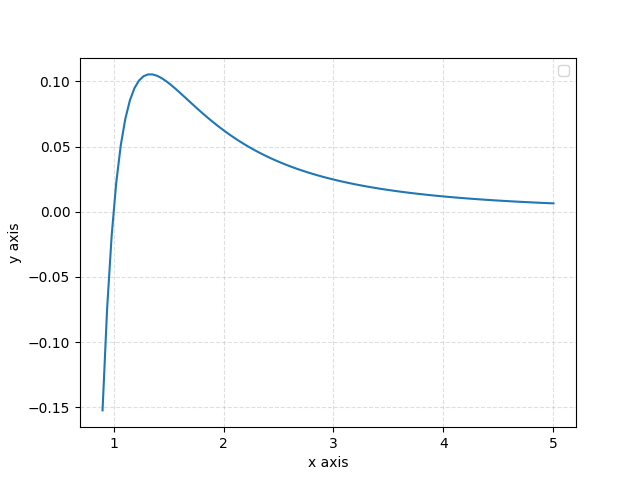
\includegraphics[clip,width=10.0cm]{graph/spherical.png}
    \caption{}
    \label{fig:spherical}
\end{figure}
ピークは
\beq
\dder[y]{x} = 
\eeq
より$x = \frac{4}{3}$のところにある。
$R$の式に代入すると、$R_m$
クリティカルマスは$M_J$

\subsubsection{自由落下時間}
ジーンズ不安定性によって崩壊が始まると、圧力勾配の上昇に比べて重力による収縮の効果が支配的になる。
一様球の崩壊において半径$r$の球殻の崩壊について考える。
半径rの球殻の内部に$m$の質量があるとすれば、球殻の運動方程式は
\beq
    \ddot{r} = - \frac{Gm}{r^2}
\eeq
と書ける。初期条件において球殻の半径が$r_0$で、一様球の密度が$\rho_0$であったとすれば$m = \frac{4\pi r_0^3}{3}\rho_0$
であるので、運動方程式は、
\beq
\ddot{r} = - \frac{4\pi Gr_0^3 \rho_0}{3r^2}
\eeq
$\dot{r}$をかけて積分すれば、初期条件において球殻が静止していたとして、
\beq
\half \dot{r}^2 = \frac{4 \pi r_0^3}{3}G\rho_0\left(\frac{1}{r} - \frac{1}{r_0} \right)
\eeq
整理すると
\beq
\frac{\dot{r}}{r_0} = \left[ \frac{8 \pi }{3}G\rho_0\left(\frac{r_0}{r} - 1\right) \right]^\half
\eeq
$\cos^2\xi = \frac{r}{r_0}$と置き換えれば、
\beq
2\dot{\xi}\cos^2\xi = \left(\frac{8\pi G \rho_0}{3} \right)^\half
\eeq
を得る。
\beq
2\dot{\xi}\cos^2\xi = \dder[]{t} \left(\xi + \half\sin 2\xi \right)
\eeq
を使って、積分すれば
\beq
\xi + \half \sin 2\xi = \left(\frac{8\pi G \rho_0}{3} \right)^\half t
\eeq
$\xi = \frac{\pi}{2}$において球殻が中心に達するので、
\beq
t_{ff} = \left(\frac{3\pi}{32\pi G \rho_0} \right)^\half
\eeq
%具体例
\subsection{Lane-Emden方程式}
星は主系列星への進化の過程で星全体での対流を経るので、星の内部の組成は主系列星に至った際には一様である。
また、星間ガスから自己重力収縮している過程も内部の組成は一様である。
%ほんと?
そこで、ここでは組成が一様な星の内部構造を調べる。まず、星が静水圧平衡にあり、ポアソン方程式が成り立つとする。
\begin{equation}
    \dder[p]{r} = - \rho\dder[\Phi]{r}\label{eq:static}
\end{equation}
\begin{equation}
    \frac{1}{r^2}\dder[]{r}(r^2\dder[\Phi]{r}) = 4\pi G\rho\label{eq:poisson}
\end{equation}
力学平衡をここまで考えたが、星の内部での電離状態を考えるには温度が必要である。
温度を与えるために、ここではエネルギー保存やエネルギー輸送の効果を考えずに、系の力学的平衡状態の性質を調べるためにポリトロープ関係式を用いる。
$K = R_{gas}T/\mu$として、
\begin{equation}
    P = K \rho^\gamma = K\rho^{1+1/n}\label{eq:polytropic}
\end{equation}
と書く。$\gamma$を比熱比、$n$をポリトロープ指数と呼ぶ。
静水圧平衡の式\eqref{eq:static}にポリトロープ関係式を代入して、
\begin{align}
    \dder[\Phi]{r} &= - \gamma K \rho^{\gamma -2} \dder[\rho]{r}\label{eq:staticpoly}
\end{align}
\subsubsection{non isothermal}
$\gamma \neq 1, n\neq \infty$のときに\eqref{eq:staticpoly}を積分して、
\begin{align}
    \Phi = \rho^{\gamma -1} (- \frac{\gamma}{\gamma -1}K)\\
    \rho = \left(- \frac{1}{n+1}\frac{\Phi}{K}\right)^n
\end{align}
を得る。$\rho =0$となるような表面では$\Phi=0$、星の内部では$\Phi < 0$であるとした。
この式を、\eqref{eq:poisson}に代入して
\begin{equation}
    \frac{1}{r^2}\dder[]{r}(r^2\dder[\Phi]{r}) = 4\pi G\left(- \frac{1}{n+1}\frac{\Phi}{K}\right)^n
\end{equation}
$\rho_c,\Phi_c$を中心密度、中心での重力ポテンシャルとして、
\begin{align}
    \rho = \rho_c \theta^n = \rho_c (\frac{\Phi}{\Phi_c})^n\\
r = a\xi, a = \left(\frac{4\pi G}{(n+1)^n K^n}(-\Phi_c)^{n-1}\right)^{1/2}
\end{align}
を使って無次元化すれば、Lane-Emden方程式\eqref{eq:laneemden}を得る。
\begin{equation}
    \frac{1}{\xi^2}\dder[]{\xi}\left(\xi^2\dder[\theta]{\xi}\right) = - \theta^n\label{eq:laneemden}
\end{equation}
この方程式の解はEmden解と呼ばれ、$\theta(\xi)$を与える。
この解は一般には初等的には求められないが、$n=5$の場合には
\beq
\theta = \frac{1}{\sqrt{1 + \frac{1}{3}\xi^2}}
\eeq
の形の解が知られている。このとき密度は
\beq
\rho =  \frac{\rho_c}{(1 + \frac{1}{3}\xi^2)^\frac{5}{2}}
\eeq
となり、これをプラマーモデルという。
\subsubsection{isothermal}
$\gamma=1,n=\infty$の等温の場合
%&= -  K \rho^{-1} \dder[\rho]{r}
\eqref{eq:staticpoly}を$\Phi=0$での密度を$\rho_c$として積分する。
\begin{align}
    - \frac{\Phi}{K} = \ln \rho - \ln \rho_c\\
    \rho = \rho_ce^{-\Phi/K}
\end{align}
これをポアソン方程式\eqref{eq:poisson}に代入すれば、
\begin{equation}
    \frac{1}{r^2}\dder[]{r}(r^2\dder[\Phi]{r}) = 4\pi G\rho_c e^{-\Phi/K}
\end{equation}
\begin{equation}
    \xi = ar, a = \left( \frac{4\pi G \rho_c}{K}\right)^{1/2}, \theta = \frac{\Phi}{K}
\end{equation}
と無次元化すると等温過程のLane-Emden方程式を得る。
\begin{equation}
    \frac{1}{\xi^2}\dder[]{\xi}\left(\xi^2\dder[\theta]{\xi}\right) = e^{-\theta}
\end{equation}
中心で密度が有限で、圧力勾配が$0$になるから、境界条件を例えば
\begin{equation}
    \theta(0) = 0,    \theta'(0) = 0
\end{equation}
とおけば、Lane-Emden方程式は解ける。
\subsection{放射}
\subsection{第一コアの形成}
重力不安定性によって重力収縮を起こしている分子雲について考える。
分子雲は崩壊を起こす前は$T=10K$で分子雲全体が等温で、かつ光学的に薄い状態である。
これは分子雲のガス粒子はダスト粒子と衝突していて、ダストの熱放射で冷却されている状態である。
この一様な分子雲が重力不安定性によって崩壊するとき、崩壊の中心部の密度が小さくダスト冷却が効く間は崩壊はほとんど$10K$の等温で進化する。
そして、中心部の密度が大きくなり、光学的に厚くなると中心部では断熱的になり急速に温度が上昇する。
輻射でエネルギーが抜けなくなった中心部のことをコアと呼ぶことにする。
コアの高密度部分の進化が暴走的に進む一方で、それを取り囲むエンベロープは一定のままである。
これは、エンベロープが中心部に質量を供給しただけ崩壊している領域の境界からエンベロープに対しても質量の流れがあることによって起きる見かけの効果とも言える。
コアの密度が上がると、自由落下時間は短くなると同時にジーンズ質量は小さくなるので
コアの質量は小さくなる。
また、コアの大きさはジーンズ長程度のまま収縮するので密度の上昇とともにエンベロープに取り残された質量の分布がわかる。
ジーンズ長が$\lambda_J \propto \rho^{-\half}$であるから、エンベロープの質量分布は
$\rho \propto r^{-2}$となる。
\subsection{解離と電離の効果}
形成された第一コアは不透明で輻射によってエネルギーが抜けない。
しかし、エンベロープからの質量降着は続くのでその重力エネルギーはコアの内部エネルギーに変換され
コアの内部の温度と圧力は上がり続ける。
温度が$2000K$に達すると、水素分子の解離の効果が現れる。
水素原子と分子の関係はSahaの式によって与えられる。
\subsubsection{Sahaの式}
原子の励起状態には様々あるが、基底状態と励起状態の間の数密度の関係を考えるとき、熱平衡にあるガスを考えるのが良い。
ガスの中では様々な状態の原子が分布していると考えられる。
ここでは$s$番目の励起状態の統計的重みを$g_s$、状態$s$にある原子の数密度を$n_s$、基底状態からのエネルギーを$\psi_s$と書くこととする。
統計的重みは、エネルギー準位における縮退度を表す。
すると
\beq
\frac{n_s}{n_0} = \frac{g_s}{g_0}e^{-\psi_s/kT}\label{eq:bolzman}
\eeq
が成り立つ。分配関数$u$を
\beq
    u = \sum g_s e^{-\psi_s kt} 
\eeq
として、数密度$n$を
\beq
    n = \sum n_s
\eeq
と定義すれば、ボルツマン公式\eqref{eq:bolzman}は分配関数を使って書き直される。
\beq
    \frac{n_s}{n} = \frac{g_s}{u} e^{-\psi_s kt}
\eeq
中性原子が$r$個の原子を失った状態を$r$階電離原子と呼ぶ。
基底状態の$r$階電離原子がさらに電子を一つ失って$(r+1)$階電離原子になるのに必要な最小のエネルギーを$\chi_r$とする。
電離した電子が運動量$p_e$を持っているとき、電離した電子のエネルギーは$E = \chi_r + \frac{p_e}{2m_e}$となる。
ここで、$r$階電離原子と自由電子が$[p_e, p_e + dp_e]$の間の運動量を持つ$r+1$階電離原子との関係を考える。
数密度はそれぞれ、$n_r, dn_{r+1}$と書く。統計的重みは、$g_r, g_{r+1}dg(p_e)$となる。
ここで$dg(p_e)$は、
プランク定数を使って
\beq
dg(p_e) = \frac{2dVd^3p_e}{h^3}
\eeq
と書かれる。ボルツマン公式は
\beq
\frac{dn_{r+1}}{n_r} = \frac{g_{r+1}dg(p_e)}{g_r} \exp\left(- \frac{\chi_r + \frac{p_e^2}{2m_e}}{kT}\right)
\eeq
$dV = \frac{1}{n_e}$であること、$[p_e, p_e + dp_e]$の空間$d^3p_e = 4\pi p_e^2 dp_e$を使って
\beq
dg(p_e) = \frac{8\pi p_e^2dp_e}{n_eh^3}
\eeq
と書けるので、
%todo:ちゃんとかく
\beq
\frac{dn_{r+1}}{n_r} = \frac{g_{r+1}}{g_r}\frac{8\pi p_e^2dp_e}{n_eh^3} \exp\left(- \frac{\chi_r + \frac{p_e^2}{2m_e}}{kT}\right)
\eeq
$p_e$について積分すれば
\beq
\frac{n_{r+1}}{n_r} n_e = \frac{g_{r+1}}{g_r} f_r(T)
\eeq
\beq
f_r(T) = 2 \frac{(2\pi m_e kT)^{\frac{3}{2}}}{h^3} e^{-\chi_r/kT}
\eeq
これをSahaの四季と呼ぶ
\subsection{2nd}
\section{衝撃波}
\subsection{衝撃波}
\subsubsection{ランキンユゴニオ}
\subsection{衝撃波の性質}
\subsection{エントロピージャンプ}
\subsection{衝撃波の大きさ}
\section{計算手法}
\subsection{差分方程式についての一般論}
\subsection{クーラン条件}
\begin{equation}
    \pder[u]{t} + c\pder[u]{x} = 0\label{eq:advection}
\end{equation}
波の伝播を表す線形移流方程式について考える。
移流速度を$c$として方程式は\eqref{eq:advection}のようになる。
この方程式の解は、$u = f(x -ct)$の形で得られ、
$c>0$ならば$x$の正の方向に、$c<0$ならば$x$の負の方向に伝播する解になる。
この方程式を$c>0$のときに風上差分法で差分化して数値的に解くことを考える。
上付き添字を時刻、下付き添字を座標に関するインデックスとおいて、
\begin{align}
    \frac{u^{n+1}_j - u^{n}_j}{\Delta t} = -c \frac{u^n_{j} - u^n_{j-1}}{\Delta x}
\end{align}
と書ける。したがって、$u$は時間方向において
\begin{align}
    u^{n+1}_j  =  u^{n}_j- c \Delta t\frac{u^n_{j} - u^n_{j-1}}{\Delta x}
\end{align}
と更新される。
時刻$n$での情報のみから次のステップでの物理量を計算する陽的な解法では、
$1$ステップの情報の伝達距離が格子幅を超えないという条件が課される。%todo:言い換え
したがって、情報が伝播する速さは$\frac{\Delta x}{\Delta t}$で、波の速さが$c$であるから条件は
\begin{equation}
    \frac{\Delta x}{\Delta t} \geq c
\end{equation}
これはクーラン条件と呼ばれ、Courant-Friedrichs-Lewy条件の略称としてCFL条件と書かれることもある。
クーラン数が1より小さい条件$c\frac{\Delta t}{\Delta x} \leq 1$とも言える。
例えば4次中心差分法ではクーラン条件は
%図を乗せる
\begin{equation}
  c\frac{\Delta t}{\Delta x} \leq 2
\end{equation}
となることからわかるように、条件は必ずしも$1$ではないが$1$を使えば十分である。
\subsubsection{フォン・ノイマンの安定性解析}
クーラン条件が満たされていることは、数値計算が安定であることを保障しない。
風上差分法において、安定性を考える。
%todo:波数空間の描画
$u_j(j=0,\cdot N)$に対して
そのフーリエ級数展開を考える。
\begin{equation}
    u^n_j = \sum_k \xi^n_k e^{ikj\Delta x}\label{eq:fourier}
\end{equation}
ここで$\xi_k$は増幅係数で、フーリエ級数の$k$番目の級数の時刻$n$における増幅率を表す。
すべてのモード$k$で$||\xi_k||\leq1$を満たすとき、数値計算が安定であるという。
方程式を差分化したものを考えて、
\begin{align}
    \frac{u^{n+1}_j - u^{n}_j}{\Delta t} =- c \frac{u^n_{j} - u^n_{j-1}}{\Delta x}
\end{align}
ここに、\eqref{eq:fourier}の波数$k$のモード$u^n_j(k) = \xi^n_ke^{ikj\Delta x}$のみを代入してみる。
すると方程式は、
\begin{align}
    (\xi_k -1)\frac{u^n_j(k)}{\Delta t}&=- \frac{c}{\Delta x} \xi^n_k(e^{ikj\Delta x} - e^{ik(j-1)\Delta x})\\
                                        &=- \frac{c}{\Delta x} u^n_j(k)e^{ikj\Delta x}(1 - e^{-ik\Delta x})
\end{align}
となり、これを$\xi_k$について解くと、$\alpha = \frac{c\Delta t}{\Delta x}$と書いて、
\begin{align}
    \xi_k &= 1 -  \alpha(1 - e^{-ik\Delta x})\\
          &= 1 - \alpha (1 - \cos(k\Delta x) + i\sin(k\Delta x))\\
    ||\xi_k||^2 &= (1 + \alpha(\cos(k\Delta x) -1))^2 + \alpha^2 \sin^2(k\Delta x)\\
                &= 1 + 2\alpha(1-\alpha)(\cos(k\Delta x) -1)
\end{align}
これは、$0 \geq \alpha \geq 1$のとき安定
%todo : くわしく
$\alpha > 1$のとき不安定である。
したがってクーラン条件が満たされるときのみ安定なスキームであるとわかった。
\subsection{人工粘性}
圧縮性流体の数値計算では衝撃波の取り扱いが必要である。
衝撃波面は数学的には2価関数が現れる不連続な現象であるが、
物理的には平均自由行程程度の厚みを持つ遷移層であるためにその前後で保存則が成り立つ。
数値計算で衝撃波を正しく取り扱わなければ、衝撃波面の前後での不連続性から保存則が成り立たず、
物理的な結果を得ることができない。
そこで1950年にvon NeumannとRichtmyer人工粘性を導入した。
人工粘性は計算に圧縮されたときのみ働く非線形な粘性で、
平均自由行程程度の大きさの衝撃波の厚みを格子の幅程度にまで大きくすることによって衝撃波を数値計算で捉えられるようにする。
そして、エネルギー方程式にも組み込まれることで、運動エネルギーを熱エネルギーへ変換する役割も果たす。
%todo:式
人工粘性無しで衝撃波を扱う方法にはLax-Wendroff法などがあり広く使われているが、
衝撃波面のまわりで解が振動するという問題も知られている。
\subsection{一次元球対称ラグランジュ座標}
\subsection{基礎方程式の差分化}
一次元の球対称ラグランジアン流体計算において、独立変数は$M_r$である。
ここで$M_r$は半径$r$の内部にある質量で定義され、媒質を外向きに大きくなる量である。
(疑似粘性の選択は注意が必要である。)
いま、解くべき方程式は
\begin{align}
    \Dder[v]{t} &= - \frac{GM_r}{r^2} - 4\pi r^2\pder[(p + Q)]{M_r}\\
    \Dder[r]{t} &= v\\
    V &= \frac{1}{\rho}=\frac{4}{3}\pder[r^3]{M_r}\\
    Q &= \frac{4}{3}\rho l^2 (\pder[v]{r})^2\label{eq:q}
\end{align}
方程式は$\left\{M_i\right\};i = 1,...,I+1$によって離散化される。
$i$番目の球殻の中の質量は
\beq
    \Delta M_{i+\half} = M_{i+1} - M_i
\eeq
陽的な差分方程式は、
\begin{align}
    \frac{v^{n+\half}_i - v^{n-\half}_i}{\Delta t^n} &= -\frac{GM_i}{(r^{n+\lambda}_i)^2}
    -4\pi(r^{n+\lambda}_i)^2
    \frac{p^{n+\lambda}_{i+\half} - p^{n+\lambda}_{i-\half}+Q^{n-\half}_{i+\half} - Q^{n-\half}_{i-\half}}{\Delta M_i}\\
    r^{n+1}_i &= r^{n}_i + v^{\hpn}_i \Delta t^{\hpn}\\
    V^{n+1}_{\hpi} &= \frac{1}{\rho^{n+1}_{\hpi}}=\frac{4}{3}\frac{(r^{n+1}_{i+1})^3 - (r^{n+1}_{i})^3}{\Delta M_{\hpi}}\\
\end{align}
途中で、
\begin{align}
    r^{n+\lambda}_i &= r^n_i + \frac{1}{4} (\Delta t^{n+\half} - \Delta t^{n-\half})v^{n-\half}_i\\
    p^{n+\lambda}_{\hpi} &=  p^{n}_{\hpi} + \frac{1}{4} (\Delta t^{n+\half} - \Delta t^{n-\half})
    \frac{p^{n}_{\hpi} - p^{n-1}_{\hpi}}{\Delta t^{\hmi}}
\end{align}
運動方程式は、
\beq
    \Dder[v]{t} = - \frac{GM_r}{r^2} - 4\pi r^2\pder[p]{M_r} - \frac{4\pi}{r}\pder[r^3Q]{M_r}
\eeq
差分化すれば、
\beq
    \frac{v^{n+\half}_i - v^{n-\half}_i}{\Delta t^n} =
    -\frac{GM_i}{(r^{n+\lambda}_i)^2}
    -4\pi(r^{n+\lambda}_i)^2
    \frac{p^{n+\lambda}_{i+\half} - p^{n+\lambda}_{i-\half}}{\Delta M_i}
    -\frac{4\pi}{r^{n}_i}
    \frac{(r^{n}_{i+\half})^3Q^{n-\half}_{i+\half} - (r^{n}_{i-\half})^3Q^{n-\half}_{i-\half}}{\Delta M_i}
\eeq
ここで、$r_{i+\half}$は質量を半分持つように選ばれる。
\begin{align}
    r_{i+\half} = (r^3_i + r^3_{i+1})^{\frac{1}{3}}
\end{align}
$Q$の更新は、
\beq
    Q^{\hmn}_{\hpi} = - 2 (\mu_Q)^{\hmn}_{\hpi}
     \left[\frac{v^{\hmn}_{i+1}-v^{\hmn}_{i}}{r^{\hmn}_{i+1}-r^{\hmn}_{i}}
      +\frac{1}{3}\frac{\ln \rho^{n}_{\hpi} - \ln \rho^{n-1}_{\hpi}}{\Delta t^{\hpn}}\right]
\eeq
粘性係数は、
\beq
    (\mu_Q)^{n-\half}_{i+\half} = 
    l^2 \frac{\left[ \rho^n_{\hpi} - \rho^{n-1}_{\hpi}\right]}{\Delta t^{\hpn}}
\eeq
ここで、$l$は
\beq
    l = k_q \Delta r
\eeq
\subsection{陰的計算}
等温の仮定を外してエネルギーを計算入れる。
放射による効果は、
\begin{align}
    l = 4\pi r^2 F\\
    F = - \frac{4ac}{3} \frac{T^3}{\kappa \rho}\pder[T]{r}
\end{align}
エネルギー方程式は、
\begin{align}
\Dder[e]{t} + p \Dder[]{t}\left(\frac{1}{\rho}\right) = \dot{q} + \Phi\\
\Dder[e]{t} + p \Dder[]{t}\left(\frac{1}{\rho}\right) = - \frac{1}{4\pi\rho r^2}\pder[l]{r} + \Phi
\end{align}    
ここで、エネルギー方程式を差分化することを考えるが、単に差分化すると2階微分が入っているので
クーラン条件が$\Delta t < \frac{\Delta x^2}{c}$となる。
時間とともに格子の幅が変化してゆく1次元ラグランジュ法を採用しているから、
この$\Delta x$は崩壊が進むとともに中心部ではジーンズ長程度まで小さくなる。
したがって、クーラン条件は崩壊の経過とともに一層厳しい条件となってしまう。
そこで、この問題を解決するために陰的な手法を導入する。
陰的な手法では、クーラン条件についての考えなくて良いのでエネルギー方程式に関するクーラン条件の問題が解決される。

\section{結果}
\subsection{等温過程における崩壊}
\subsection{断熱過程におけるコアの形成}
\subsection{輻射の効果を入れてエネルギー方程式を解く}
\subsection{解離の効果による第一コアの崩壊と第二コアの形成}
\section{結論}
\bibliographystyle{junsrt}
\bibliography{cite}
\end{document}
